%%%%%%%%%%%%%%%%%%%%%%%%%%%%%%%%%%%%%%%%%%%%%%%
%%%     Declarations (skip to Begin Document, line 88, for parts you fill in)
%%%%%%%%%%%%%%%%%%%%%%%%%%%%%%%%%%%%%%%%%%%%%%%

\documentclass[10pt]{article}

\usepackage{geometry}  % Lots of layout options.  See http://en.wikibooks.org/wiki/LaTeX/Page_Layout
\geometry{letterpaper}  % ... or a4paper or a5paper or ... 
\usepackage{fullpage}  % somewhat standardized smaller margins (around an inch)
\usepackage{setspace}  % control line spacing in latex documents
\usepackage[parfill]{parskip}  % Activate to begin paragraphs with an empty line rather than an indent
\usepackage{amsmath,amssymb}  % latex math
\usepackage{empheq} % http://www.ctan.org/pkg/empheq
\usepackage{bm,upgreek}  % allows you to write bold greek letters (upper & lower case)

\usepackage{url}

% allows strikethroughs in math via \cancel{math text goes here}
\usepackage{cancel}

% for typsetting algorithm pseudocode see http://en.wikibooks.org/wiki/LaTeX/Algorithms_and_Pseudocode
\usepackage{algorithmic,algorithm}  

\usepackage{graphicx}  % inclusion of graphics; see: http://en.wikibooks.org/wiki/LaTeX/Importing_Graphics
% allow easy inclusion of .tif, .png graphics
\DeclareGraphicsRule{.tif}{png}{.png}{`convert #1 `dirname #1`/`basename #1 .tif`.png}

%\usepackage{subfigure}  % allows subfigures in figure
\usepackage{caption}
\usepackage{subcaption}

\usepackage{xspace}
\newcommand{\latex}{\LaTeX\xspace}

\usepackage{color}  % http://en.wikibooks.org/wiki/LaTeX/Colors

\long\def\ans#1{{\color{blue}{\em #1}}}
\long\def\ansnem#1{{\color{blue}#1}}
\long\def\boldred#1{{\color{red}{\bf #1}}}
\long\def\boldred#1{\textcolor{red}{\bf #1}}
\long\def\boldblue#1{\textcolor{blue}{\bf #1}}
\long\def\todo#1{\textcolor{red}{\bf TODO: #1}}

% Useful package for syntax highlighting of specific code (such as python) -- see below
\usepackage{listings}  % http://en.wikibooks.org/wiki/LaTeX/Packages/Listings
\usepackage{textcomp}

%%% The following lines set up using the listings package
\renewcommand{\lstlistlistingname}{Code Listings}
\renewcommand{\lstlistingname}{Code Listing}

%%% Specific for python listings
\definecolor{gray}{gray}{0.5}
\definecolor{green}{rgb}{0,0.5,0}

\lstnewenvironment{python}[1][]{
\lstset{
language=python,
basicstyle=\footnotesize,  % could also use this -- a little larger \ttfamily\small\setstretch{1},
stringstyle=\color{red},
showstringspaces=false,
alsoletter={1234567890},
otherkeywords={\ , \}, \{},
keywordstyle=\color{blue},
emph={access,and,break,class,continue,def,del,elif ,else,%
except,exec,finally,for,from,global,if,import,in,i s,%
lambda,not,or,pass,print,raise,return,try,while},
emphstyle=\color{black}\bfseries,
emph={[2]True, False, None, self},
emphstyle=[2]\color{green},
emph={[3]from, import, as},
emphstyle=[3]\color{blue},
upquote=true,
morecomment=[s]{"""}{"""},
commentstyle=\color{gray}\slshape,
emph={[4]1, 2, 3, 4, 5, 6, 7, 8, 9, 0},
emphstyle=[4]\color{blue},
literate=*{:}{{\textcolor{blue}:}}{1}%
{=}{{\textcolor{blue}=}}{1}%
{-}{{\textcolor{blue}-}}{1}%
{+}{{\textcolor{blue}+}}{1}%
{*}{{\textcolor{blue}*}}{1}%
{!}{{\textcolor{blue}!}}{1}%
{(}{{\textcolor{blue}(}}{1}%
{)}{{\textcolor{blue})}}{1}%
{[}{{\textcolor{blue}[}}{1}%
{]}{{\textcolor{blue}]}}{1}%
{<}{{\textcolor{blue}<}}{1}%
{>}{{\textcolor{blue}>}}{1},%
%framexleftmargin=1mm, framextopmargin=1mm, frame=shadowbox, rulesepcolor=\color{blue},#1
framexleftmargin=1mm, framextopmargin=1mm, frame=single,#1
}}{}
%%% End python code listing definitions

\DeclareMathOperator{\diag}{diag}
\DeclareMathOperator{\cov}{cov}

%%%%%%%%%%%%%%%%%%%%%%%%%%%%%%%%%%%%%%%%%%%%%%%
%%%     Begin Document
%%%%%%%%%%%%%%%%%%%%%%%%%%%%%%%%%%%%%%%%%%%%%%%

\begin{document}

\begin{center}
    {\Large {\bf ISTA 421 / INFO 521 -- Final Project OPTION A: Metropolis-Hastings MCMC Inference of 3D Line}} \\
    \boldred{Due: Friday, December 8, 8pm} \\
    Total 20\% of final grade \\
    \vspace{1cm}
    %{\Large \boldblue{Solutions}}
\end{center}

\begin{flushright}
STUDENT NAME %% Fill in your name here

Undergraduate / Graduate %% select which you are!
\end{flushright}

\section*{Introduction}

The following are the instructions for Option A of the final project. If you are doing Option B, you do NOT do this option; you should instead refer to the instructions for Option B.

The instructions start with a general background description of the model and problem scenario, followed by a set of Tasks. You must commit and push your executable code along with a PDF of written answers to your final\_project repository. The name of your written PDF must be {\tt final\_project\_OptionA\_answers.pdf}. The first task has you implement the core code to your Metropolis-Hastings sampler. Tasks 2 through 5 then require you to run that code on the provided data in various configurations, generate plots, report values, and describe the outcomes.

%%%     Option A
\section*{Option A Background: Inferring parameters of a 3D line from noisy 2D images using Metropolis-Hastings MCMC}

In vision problems, we often represent the process by which an image is produced by considering a parameterized camera model (in a sense, the camera model defines the ``perspective'' toward the scene) and the scene being imaged.

In the pinhole camera model, cameras can be represented by matrices that contain parameters for the camera, such as its position in space and its focal length.\footnote{For those interested ({\em not} required for this project), details can be found in Hartley and Zisserman (2004) {\em Multiple View Geometry in Computer Vision}; you can also internet search for ``camera matrix.''}  This representation is useful because it allows us to obtain 2D images of 3D points in a very simple way.

Let $\mathbf{M} \in \mathbb{R}^{3 \times 4}$ be a camera matrix.  Then, if $\mathbf{p} \in \mathbb{R}^3$ is a 3D point (i.e., $\mathbf{p} = [p_1, p_2, p_3]^{\top}, p_i \in \mathbb{R}$), its 2D image $\mathbf{q} \in \mathbb{R}^2$ is given by
\begin{eqnarray}
\mathbf{q} = 
\begin{bmatrix}
u \\ v
\end{bmatrix}
= \frac{1}{\widetilde{w}}
\begin{bmatrix}
\widetilde{u} \\ \widetilde{v}
\end{bmatrix}
\label{eqn:q}
\end{eqnarray}
where $\widetilde{u}$, $\widetilde{v}$, and $\widetilde{w}$ are defined by
\begin{eqnarray}
\begin{bmatrix}
\widetilde{u} \\ \widetilde{v} \\ \widetilde{w}
\end{bmatrix}
= \mathbf{M}
\begin{bmatrix}
\mathbf{p} \\ 1
\end{bmatrix}
= \mathbf{M}
\begin{bmatrix}
p_1 \\ p_2 \\ p_3 \\ 1
\end{bmatrix}
\label{eqn:p-proj-to-q}
\end{eqnarray}
Notice the number 1 that is appended to $\mathbf{p}$ when multiplying by $\mathbf{M}$.  This is called the {\em homogeneous} coordinate, and it is necessary for posing camera projections as matrix multiplication.  This projection principle is illustrated in Figure~\ref{fig:projections}

\begin{figure}
\centering
\begin{subfigure}{.4\textwidth}
  \centering
  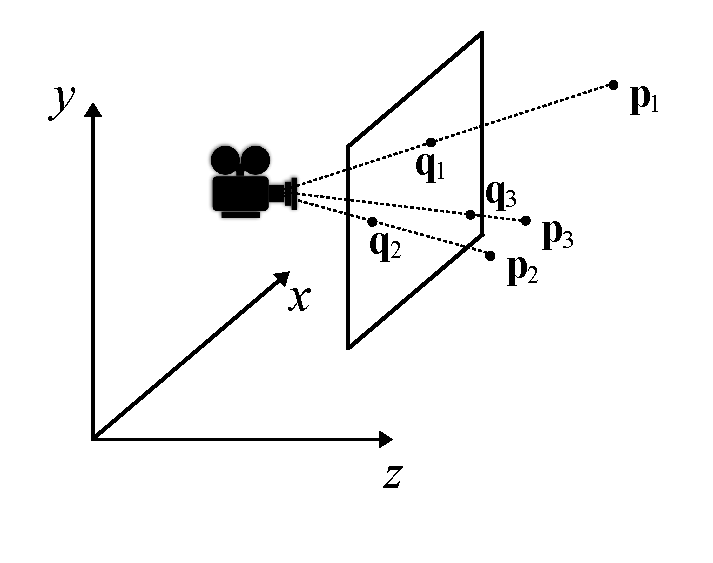
\includegraphics[width=1\linewidth]{figures/camera-projection-3d}
  \caption{A depiction of the projection of three points $\mathbf{p}_1$, $\mathbf{p}_2$, $\mathbf{p}_3 \in \mathbb{R}^3$ onto the image plane of a camera using Eqs~\ref{eqn:q}~and~\ref{eqn:p-proj-to-q}.}
  \label{fig:3d}
\end{subfigure}%
\hspace{1cm}
\begin{subfigure}{.4\textwidth}
  \centering
  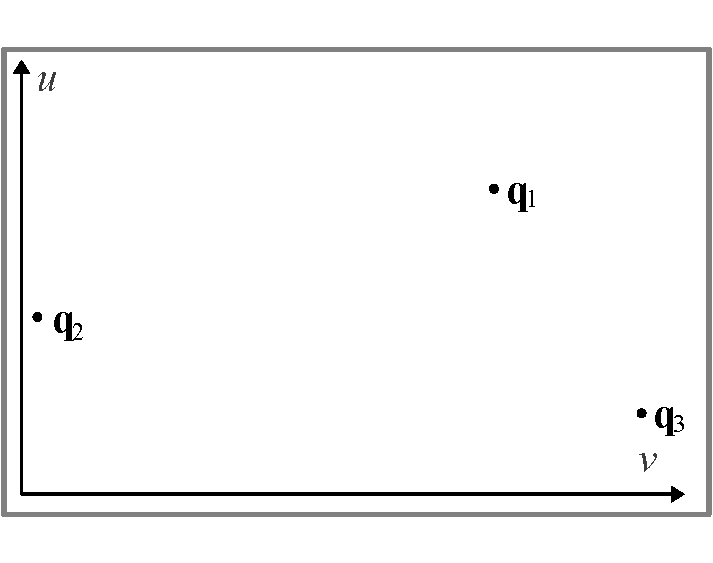
\includegraphics[width=1\linewidth]{figures/camera-projection-2d}
  \caption{Graphical depiction of the 2D image plane with image points $\mathbf{q}_1$, $\mathbf{q}_2$, $\mathbf{q}_3 \in \mathbb{R}^2$ projected from points $\mathbf{p}_1$, $\mathbf{p}_2$, and $\mathbf{p}_3$.}
  \label{fig:2d}
\end{subfigure}
\caption{Two views of projection.\label{fig:projections}}
\end{figure}

{\em NOTE: A complete understanding of this material, while very valuable in itself (!), is not necessary to complete this problem.}  The only thing you are required to understand is that 3D points (in coordinates $x$, $y$ and $z$ of Figure~\ref{fig:projections}a) become 2D image pixel points (in coordinates $u$, $v$ of Figure~\ref{fig:projections}b) by Equations~\ref{eqn:q}~and~\ref{eqn:p-proj-to-q}.

We will start by defining a ``Camera 1'' whose matrix is
\begin{eqnarray*}
\mathbf{M} = 
\begin{bmatrix}
1 & 0 & 0 & 0 \\
0 & 1 & 0 & 0 \\
0 & 0 & 1 & 0
\end{bmatrix}.
\end{eqnarray*}
Camera 1 corresponds to a camera located at world coordinates $(0,0,0)$ and pointing down the positive $z$-axis, with unit focal length.  What follows is the problem setup.

Let $\boldsymbol{\ell} = (\mathbf{p}_i, \mathbf{p}_f)$ be a 3D line segment with end-points $\mathbf{p}_i, \mathbf{p}_f \in \mathbb{R}^3$.  (The subscripts on the end-points stand for ``initial'' and ``final'', respectively.)  Now, consider the following generative process.  We ``take a picture'' of $\boldsymbol{\ell}$ using camera $\mathbf{M}$, producing $\boldsymbol{\ell}_{2D} = (\mathbf{q}_{i}, \mathbf{q}_{f})$ (that is, the $\mathbf{q}_{i}$ and $\mathbf{q}_{f}$ are obtained using Equations~\ref{eqn:q}~and~\ref{eqn:p-proj-to-q}).  

We then sample $S$ points $\mathbf{q}_s$ from the line $\boldsymbol{\ell}_{2D}$.  This is accomplished by taking the ratios $t_1, ..., t_S$ along the straight-line path from $\mathbf{q}_{i}$ to $\mathbf{q}_{f}$ so that $\mathbf{q}_s = \mathbf{q}_i + (\mathbf{q}_f - \mathbf{q}_i)t_s$, with $0 \leq t_s \leq 1$, $s = 1, ..., S$. (Figure~\ref{fig:line-gen}(b) shows one of these sampled points, $\mathbf{q}_m$, which happens to be exactly half way between $\mathbf{q}_{i}$ and $\mathbf{q}_{f}$, so for this point $t_m=0.5$).  

In our scenario, the imaging and rendering processes are inherently noisy, so we add Gaussian noise to the $\mathbf{q}_s$, which gives us $\mathbf{r}_s = \mathbf{q}_s + \boldsymbol{\epsilon}$, where $\boldsymbol{\epsilon} \sim \mathcal{N}(\mathbf{0}, \boldsymbol{\Sigma})$, with $\boldsymbol{\Sigma}$ a $2 \times 2$ covariance matrix (since this noise is in the 2D image plane).  Naturally, this implies that $\mathbf{r}_s | \mathbf{p}_i, \mathbf{p}_f, t_s, \boldsymbol{\Sigma} \sim \mathcal{N}(\mathbf{q}_s, \boldsymbol{\Sigma})$.  See Figure~\ref{fig:line-gen} for a summary illustration of the generative process. 

\begin{figure}
\centering
\begin{subfigure}{.4\textwidth}
  \centering
  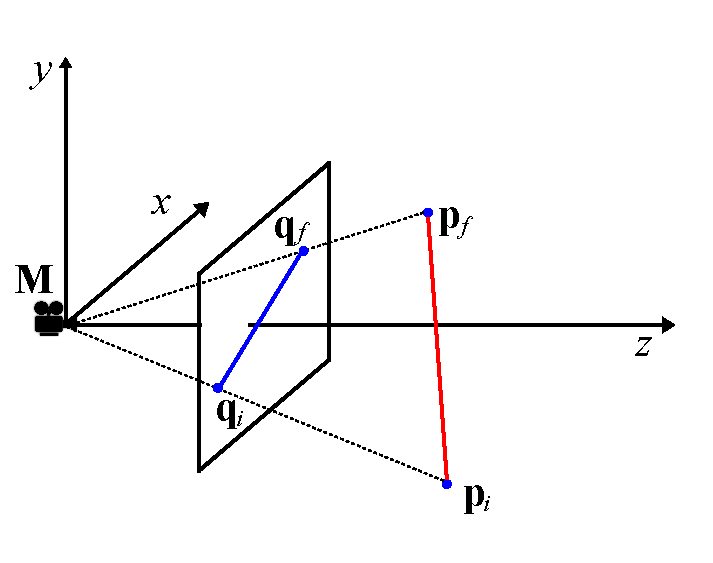
\includegraphics[width=1\linewidth]{figures/line-projection-3d}
  \caption{A 3D line segment $\boldsymbol{\ell} = (\mathbf{p}_i, \mathbf{p}_f)$ (in red) projected onto the image {\em via} camera $\mathbf{M}$ (situated at the origin), producing a (non-noisy) 2D line $\mathbf{l}_{2D} = (\mathbf{q}_i, \mathbf{q}_f)$ (in blue).}
  \label{fig:3d}
\end{subfigure}%
\hspace{1cm}
\begin{subfigure}{.4\textwidth}
  \centering
  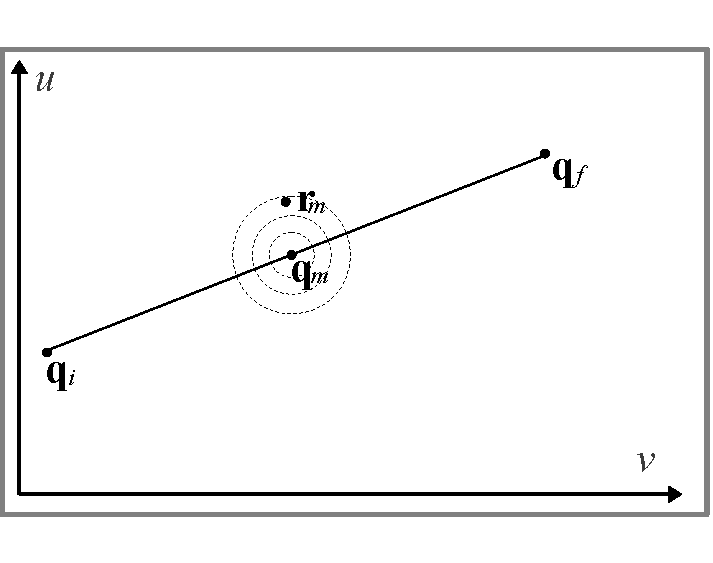
\includegraphics[width=1\linewidth]{figures/line-projection-2d}
  \caption{Image of $\boldsymbol{\ell}_{2D} = (\mathbf{q}_i, \mathbf{q}_f)$ of the projected 3D line segment in the camera $u$,$v$ plane; $\mathbf{q}_m$ is one of the sampled points along the line, which has noise, $\epsilon$, added to it in the image-creation process, generating the observed image point $\mathbf{r}_m$; the concentric circles around $\mathbf{q}_m$ represent the contours of the 2D Gaussian noise, $\boldsymbol{\epsilon}$.}
  \label{fig:2d}
\end{subfigure}
\caption{The noisy generative process projecting end-points along the line to the image\label{fig:line-gen}.}
\end{figure}

We will additionally place a Gaussian prior on the possible end-points, $\mathbf{p}_i, \mathbf{p}_f$, of the line $\boldsymbol{\ell}$ (this is a {\em different} Gaussian than the image Gaussian noise $\boldsymbol{\epsilon}$).  These prior parameters are subscripted by the bold-$\boldsymbol{\ell}$ to indicate they refer to the properties of the 3D line.  This represents the prior belief about where the line, as defined by end-points $\mathbf{p}_i$ and $\mathbf{p}_f$, might be in 3D space:
\begin{eqnarray*}
\mathbf{p}_i, \mathbf{p}_f \sim \mathcal{N}(\boldsymbol{\mu}_{\boldsymbol{\ell}}, \boldsymbol{\Sigma}_{\boldsymbol{\ell}}) .
\end{eqnarray*}

\newpage
\section*{Tasks [34 points total]}


All data files needed for this task are provided in {\tt projectA-3D-line-MH/data\_2023/}

For this project option, you will need to complete the following five tasks:

\begin{enumerate}

\item {\bf [10 points]} Write a python script that, given
\begin{itemize}
\item inputs $t_1, ..., t_S$ (the relative offset ratios of points $\mathbf{q}_s$ along the line segment between the $\mathbf{q}_i$ and $\mathbf{q}_f$ endpoints),
\item 2D points $\mathbf{r}_1, ..., \mathbf{r}_S$ (the observed points in the camera $u$,$v$ image plane),
\item $\boldsymbol{\Sigma}$ (the image projection noise covariance),
\item $\boldsymbol{\mu}_{\boldsymbol{\ell}}$ and $\boldsymbol{\Sigma}_{\boldsymbol{\ell}}$ (the priors over the 3D line segment endpoints),
\end{itemize}
uses the Metroplis-Hastings (M-H) algorithm to sample from the posterior of $\mathbf{p}_i$ and $\mathbf{p}_f$.  In other words, the script should generate samples of $\mathbf{p}_i$ and $\mathbf{p}_f$ according to the posterior distribution
\begin{eqnarray*}
p(\mathbf{p}_i, \mathbf{p}_f | \mathbf{r}, \mathbf{t}, \boldsymbol{\Sigma}, \boldsymbol{\mu}_\mathbf{l}, \boldsymbol{\Sigma}_\mathbf{l}) 
\propto 
p(\mathbf{r} | \mathbf{p}_i, \mathbf{p}_f, \mathbf{t}, \boldsymbol{\Sigma})
p(\mathbf{p}_i, \mathbf{p}_f | \boldsymbol{\mu}_\mathbf{\ell}, \boldsymbol{\Sigma}_\mathbf{\ell}),
\end{eqnarray*}
with $\mathbf{r} = \{\mathbf{r}_1, ..., \mathbf{r}_S \}$ and $\mathbf{t} = \{t_1, ..., t_S \}$.

NOTE: The prior and likelihood probabilities can be {\em extremely} small, to the point that their product can result in floating-point number underflow errors -- i.e., the computer cannot represent the small values and so treats them as though they were zero. This particularly becomes a hazard when you take the product of two very small numbers, which can happen when computing the posteriors in the M-H acceptance ratio, which in turn can lead to ``division by zero'' errors (when the denominator of the acceptance ratio is treated as zero).  A work-around is to take the $\log$ (remember, we follow the machine learning convention that this is really the {\em natural log}) of the acceptance ratio (be sure to compute the $\log$ completely through the ratio and products), do your numeric computations to get the log-ratio $\alpha$. You then have two options for how you can use this log-ratio $\alpha$:
\begin{itemize}
\item You can transform the final value back into the original scale by computing $e^{\alpha}$, and then compute your acceptance test;
\item {\em or} keep it in the log scale. If you do this, you must also ensure your random sample is also log scale! For this, the python function {\tt scipy.stats.multivariate\_normal.logpdf} will be handy. Also, keep in mind that when you perform your acceptance test, that must also be considered in the log-scale.
\end{itemize}

The written answer for this task (task 1) requires that you describe how to run your script for the following 4 tasks (tasks 2 through 5). As you complete the following tasks, you should update you description here.

\item {\bf [6 points]} \label{task-b} Use your script to draw samples from the posterior distribution of the 3D line segment end-points. 

The observations you will use in this task are taken from the perspective of Camera 1 only.
As described above, the observations consist of points $\mathbf{r}_s$ in the $u$,$v$ image plane of the camera that result from a noisy projection process originating from points $\mathbf{q}_s$. % that are themselves along the projection of the 3D line segment into the $u,v$ image plane.
Each $\mathbf{q}_s$ was itself sampled some relative offset $t_s$ (relative to the segment endpoints, $\mathbf{q}_i$ and $\mathbf{q}_f$). The data file {\tt inputs.csv} contains the relative offset ratios for each $\mathbf{q}_s$. 
The projection of point $\mathbf{q}_s$, however, is not directly observed, but instead appears in the $u$,$v$ image plane as the result of a noisy process (Figure~\ref{fig:line-gen}(b)) that produces the observed point $\mathbf{r}_s$ in the $u$,$v$ image plane coordinates. The $u$,$v$ coordinates of each of these observations are contained in the data file {\tt points\_2d\_camera\_1.csv}. (The row indices of the offset ratios in {\tt inputs.csv} corresponds to the row indices of the points in {\tt points\_2d\_camera\_1.csv}.)

Assume the following prior parameters: $\boldsymbol{\Sigma}_{\boldsymbol{\ell}} = 6 \cdot \mathbf{I}_{3 \times 3}$ (where here $\mathbf{I}_{3 \times 3}$ is the $3 \times 3$ identity matrix), $\boldsymbol{\mu}_{\boldsymbol{\ell}} = [0,0,6]^{\top}$.

Also assume that $\boldsymbol{\Sigma} = (0.05)^2 \cdot \mathbf{I}_{2 \times 2}$ (where here $\mathbf{I}_{2 \times 2}$ is the $2 \times 2$ identity matrix and $(0.05)^2$ is the scalar value of the square of $0.05$).  

It is recommended that you sample your initial end-points from the prior.  Sample for $50,000$ iterations.  

It is up to you to choose your proposal distribution! You may need to try some different parameterizations to get a good one.

Note: you will likely find your best (MAP) fit points within the first 3,000-5,000 samples, but you should sample for $50,000$ to see what the longer-term trend in your estimates looks like.

In your written answers for this task, including the following: 
\begin{itemize}
\item (3 points) Generate a plot like that of Figure 4.12(c), page 161 of FCML (2nd edition), for each parameter you are estimating, to view progress during sampling.  Remember, only plot the {\em accepted} samples, not the rejected samples. Provide informative captions.


\item (3 points) Describe the trends you see in these plots, and include an explanation of what they are telling you.  Expect to see some differences between the plots you generate and what you see in FCML Figure 4.12(c).


\end{itemize}

\item {\bf [4 points]} \label{task-c} Using the samples you generated, find the maximum a posteriori (MAP) estimate of the line end-points.
Report your results, including: 
\begin{itemize}
\item (1 point) Report your MAP estimate of the line end-points (the 3d points of each endpoint).


\item (3 points) Plot the MAP estimate of the line (that is, the MAP for each endpoint with a line connecting them) as projected onto the Camera 1 image plane (using the Camera 1 camera matrix). Include in the plot the original noisy observations, $\mathbf{r}$, of points sampled along the true line. You should see that your inferred line fits fairly well among the points. If not, try running your M-H procedure again with a different starting point for your line end-points (it is generally a good idea to sample your first end-points from the prior; update your plots in task 2 if you re-run, so that what you report there corresponds to the same data that you report here). Include in your caption an explanation for what is plotted.


\end{itemize}

\item \label{task-e} {\bf [4 points]} Suppose we have a second camera
\begin{eqnarray*}
\mathbf{M}^{\prime} =
\begin{bmatrix}
0 & 0 & 1 & -5 \\
0 & 1 & 0 & 0 \\
-1 & 0 & 0 & 5
\end{bmatrix} ,
\end{eqnarray*}
(a camera at $[5, 0, 5]^{\top}$ looking in the negative $x$-axis and unit focal length), 
and, consequently, a second set of observed data points $\mathbf{r}^{\prime}_1, ..., \mathbf{r}^{\prime}_S$, where the indices of these points correspond to the same points viewed from the first camera (those were provided in {\tt points\_2d\_camera\_1.csv}), but now we have what those points look like through the second camera, as found in {\tt points\_2d\_camera\_2.csv}.  First, let's see how your estimate from task~\ref{task-b} looks from this second camera:
\begin{itemize}
\item Create another plot like you did in task~\ref{task-c}, where you plotted the MAP hypothesis of the end-points sampled in task~\ref{task-b}, but instead use the second camera matrix to project your MAP hypothesis of the end-points (still connect them by a line), and also plot the new views of the points along the line from the perspective of the second camera, as found in {\tt points\_2d\_camera\_2.csv}. Include in your caption an explanation of what is plotted, and how it compares to the plot for Camera 1.


\end{itemize}

\item {\bf [10 points]} \label{task-f} Now, perform M-H sampling again, but this time use the data from {\bf both} cameras.  You will need to adapt your likelihood to now consider the two camera data sources, but the rest of M-H stays the same!  Again, $50,000$ iterations in M-H should be sufficient to converge and to see the longer-term trend.
Report the following:
\begin{itemize}
\item (2 points) Find and report the MAP estimate of the line using the same setup as in task~\ref{task-b} using both the observations in {\tt points\_2d\_camera\_1.csv} from the first camera and the points {\tt points\_2d\_camera\_2.csv} viewed by the second camera.


\item (4 points) Make the same plots that you did in task~\ref{task-b}.  Do they qualitatively look the same as those from task~\ref{task-b}?  If they're different, describe how and offer an explanation as to why we see those differences.


\item (4 points) Plot the projection of your {\bf new} MAP end-points estimate for the combined cameras; make one plot each for the projection of your MAP end-points connected by a line for Camera 1 (along with the noisy data for that camera), and another for Camera 2.  How well do you fit the points in both camera projections?


\end{itemize}

\end{enumerate}

\end{document}

